\subsection{Metodología de Investigación}

Este proyecto se enmarca dentro de una metodología de investigación aplicada de base tecnológica, dado que se centra en la migración e implementación de una infraestructura tecnológica avanzada para una organización real, aplicando conocimientos previos en nuevas condiciones y validando soluciones en entornos operativos. En este tipo de investigación, el conocimiento se genera a partir de la aplicación práctica de soluciones técnicas, con énfasis en el desarrollo, validación y mejora de tecnologías existentes, más que en la formulación de teorías abstractas.

Como se puede apreciar en la \autoref{fig:tlr_levels}, se hace uso del enfoque de Niveles de Maduración Tecnológica (TLR) --\textit{Technology Readiness Level}, por sus siglas en inglés-- adoptado por Colciencias para definir el alcance y la madurez tecnológica de actividades que tienen que ver con Investigación, Desarrollo Tecnológico e Innovación ($I+D+i$) en el Sistema Nacional de Ciencia, Tecnología e Innovación (SNCTeI) en Colombia \cite{Colciencias2016}.

\newcommand\tlrLevelsCaption{actividades de $I+D+i$ y otras actividades. \hspace{1em}}

\begin{figure}[H]
  \centering
  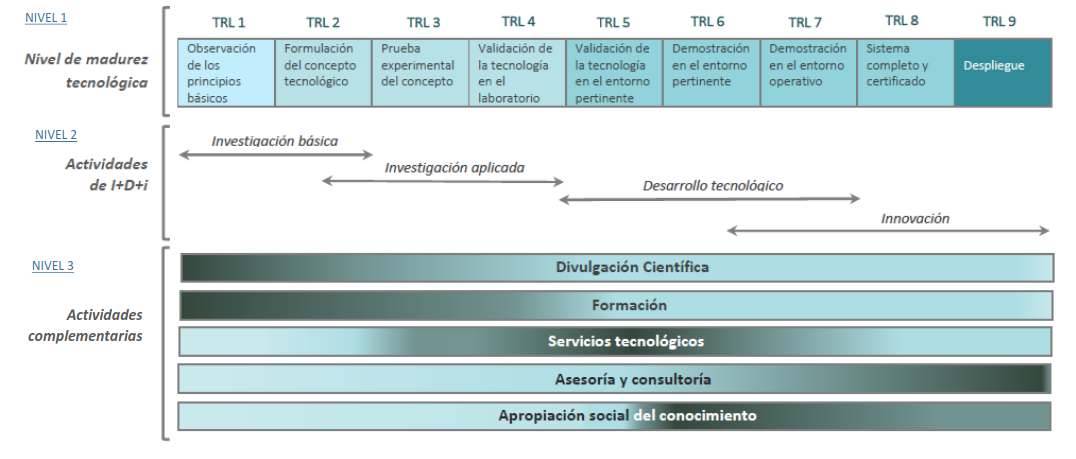
\includegraphics[width=1\textwidth]{img/figures/fig8-TLR-explanation.png}
  \caption[\tlrLevelsCaption]{\tlrLevelsCaption Fuente: Tomado de \cite{Colciencias2016}}
  \label{fig:tlr_levels}
\end{figure}

Los proyectos de software como Paralegales se ubican en los niveles más altos de madurez tecnológica: TRL 7 a TRL 9, correspondientes a las fases de investigación aplicada, desarrollo tecnológico e innovación. En estos niveles se realiza la demostración de la tecnología en entornos operativos, la validación completa del sistema y su despliegue final en condiciones reales de funcionamiento.

Esta clasificación refleja con claridad el tipo de trabajo que se está llevando a cabo: una solución concreta que busca resolver problemas técnicos y operativos reales en una organización, a través de la aplicación de buenas prácticas de ingeniería de software, la integración de servicios tecnológicos avanzados y la validación continua en producción.

Por otro lado, la investigación se puede clasificar como \textit{``in vivo''} pues se desarrolla en una organización real \cite{ChavarriagaLIDIS}. Además, se opta por la estrategia de investigación definida por Chavarriaga y Arboleda, basada en los modelos de Martin y McClure, y del SEI (\textit{Software Engineering Institute}), la cual consiste en tres etapas: (1) investigación y desarrollo inicial, (2) Investigación aplicada, y (3) Transferencia \cite{ChavarriagaLIDIS,ChavarriagaModelo}.

\newcommand\arboledaChavarriagaMetodologiaCaption{Esquema de la estrategia de investigación propuesto por Chavarriaga y Arboleda. \hspace{1em}}
\begin{figure}[H]
  \centering
  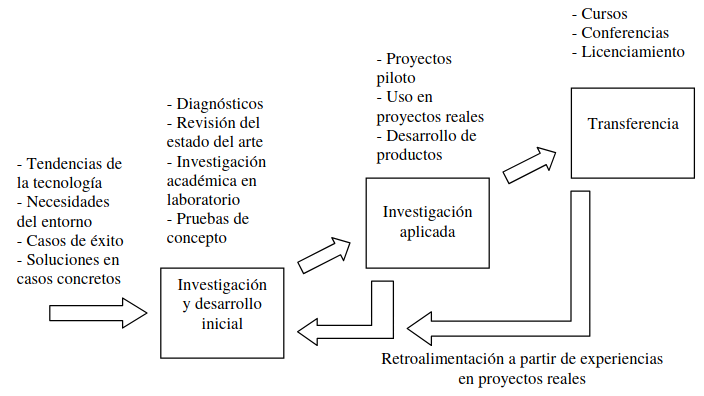
\includegraphics[width=0.8\textwidth]{img/figures/fig9-chavarriaga-arboleda.png}
  \caption[\arboledaChavarriagaMetodologiaCaption]{\arboledaChavarriagaMetodologiaCaption Fuente: Tomado de \cite{ChavarriagaLIDIS}}
  \label{fig:arboleda-chavarriaga-metodologia}
\end{figure}

Como se puede apreciar en la \autoref{fig:arboleda-chavarriaga-metodologia}, el modelo parte de una fase inicial en la que se realiza un diagnóstico, revisión del estado del arte y pruebas de concepto, seguida de una etapa de investigación aplicada donde se desarrollan soluciones en escenarios reales, y finalmente se alcanza la fase de transferencia, en la cual los conocimientos y productos generados son compartidos a través de formación, licenciamiento o difusión. Esta secuencia metodológica resulta pertinente para el presente proyecto, dado que:

\begin{enumerate}
  \item Se parte de necesidades concretas del entorno (el caso de Paralegales y su infraestructura actual).
  \item Se aplican tecnologías maduras mediante pruebas controladas y despliegues en producción.
  \item Se espera generar una solución replicable, que pueda ser transferida como buena práctica en entornos similares.
\end{enumerate}

En este sentido, el proyecto no se limita al desarrollo técnico, sino que busca una contribución tecnológica efectiva, orientada a la solución de un problema real, con posibilidad de transferencia y aprovechamiento del conocimiento en otros contextos organizacionales o académicos.
